\documentclass[10pt,aspectratio=43]{beamer}
\usetheme{Berlin}

\usepackage{amsmath,bm,amsfonts,amssymb,enumerate,graphicx,animate,epsfig,bbm,calc,color,ifthen,capt-of,multimedia}
\usepackage{fancybox,xcolor,booktabs,colortbl}
\usepackage{physics}
\usepackage{../mycommand}%我惯用的命令,在本project中,存储在本文件的父文件夹
\graphicspath{{figures/}}

\usefonttheme{professionalfonts}
\usepackage[UTF8,fontset=none,scheme=chinese]{ctex}
\setmainfont{Times}
\setsansfont{Arial}
\setmonofont{Consolas}
\setCJKmainfont{SimSun}[BoldFont=SimHei,ItalicFont=KaiTi]
\setCJKsansfont{SimHei}
\setCJKmonofont{Microsoft YaHei}
\usepackage{unicode-math}
\setmathfont{XITS Math}

\usepackage{../beamercolorthemesustech}%效果同\usecolortheme{sustech},但\usecolortheme不支持自由选择文件路径,故调用底层的\usepackage命令
\definecolor{mygreen}{rgb}{0,0.6,0}
\definecolor{mymauve}{rgb}{0.58,0,0.82}
\definecolor{mygray}{gray}{.9}
\definecolor{mypink}{rgb}{.99,.91,.95}
\definecolor{mycyan}{cmyk}{.3,0,0,0}

\usepackage[ruled,linesnumbered]{algorithm2e}
\usepackage{verbatim,listings}
\lstset{ %
	backgroundcolor=\color{white},   % choose the background color
	basicstyle=\footnotesize\ttfamily,     % size of fonts used for the code
	columns=fullflexible,
	breaklines=true,                 % automatic line breaking only at whitespace
	captionpos=b,                    % sets the caption-position to bottom
	tabsize=4,
	commentstyle=\color{mygreen},    % comment style
	escapeinside={\%*}{*)},          % if you want to add LaTeX within your code
	keywordstyle=\color{blue},       % keyword style
	stringstyle=\color{mymauve}\ttfamily,     % string literal style
	numbers=left, 
	%	frame=single,
	rulesepcolor=\color{red!20!green!20!blue!20},
	% identifierstyle=\color{red},
	language=c
}

\setbeamertemplate{caption}[numbered]%添加图片的编号
\setbeamertemplate{sidebar right}{}%去掉默认添加的navigarion symbols
\setbeamercovered{transparent}%使未点出来的文字呈现透明,默认0.15透明度
\beamerdefaultoverlayspecification{}

\usepackage[backend=biber,bibstyle=gb7714-2015,citestyle=verbose]{biblatex}
\addbibresource{../reference.bib}

%题目,作者,学校,日期
\title{Boundedness and Stability}
\subtitle{\fontsize{9pt}{14pt}\textbf{第八次\quad SDEM 5.6}}
\author{杨徵羽}
%\institute{哈尔滨工业大学(威海)理学院}
\date{\today}

\begin{document}

\frame{\titlepage}

\begin{frame}{全章结构}
\begin{table}[htbp]%\caption{全章结构}\label{t1}\centering
\resizebox{\columnwidth}{!}{
\begin{tabular}{cccccc}
\toprule
稳定性种类 & 节 & 定义 & V函数判别法 & 系数判别法 & 例子 \\
\midrule
p阶矩渐近有界 & 5.2 & 1 & 2 & 3 & 4,5 \\
p阶矩指数稳定 & 5.3 & 7 & 8 & 10,12,16 & 25,26,27 \\
p阶矩渐近稳定 & 5.4 & 28 & 29,30,31 &  & 32,33 \\
a.s.指数稳定 & 5.3 & 7 & 9 & 10,12,13,14,16 &  \\
a.s.渐近稳定 & 5.4 & 28 & 29 &  &  \\
依概率稳定 & 5.5 & 34 & 35 &  &  \\
依概率渐近稳定 & 5.5 & 34 & 36 &  & 38 \\
依概率渐近大范围稳定 & 5.5 & 34 & 37 &  &  \\
依分布渐近稳定 & 5.6 & 40 & 43 & 44 & 45,46 \\
\bottomrule
\end{tabular}
}
\end{table}
\end{frame}

\begin{frame}{5.6 Asymptotic Stability in Distribution}
\begin{figure}
\centering
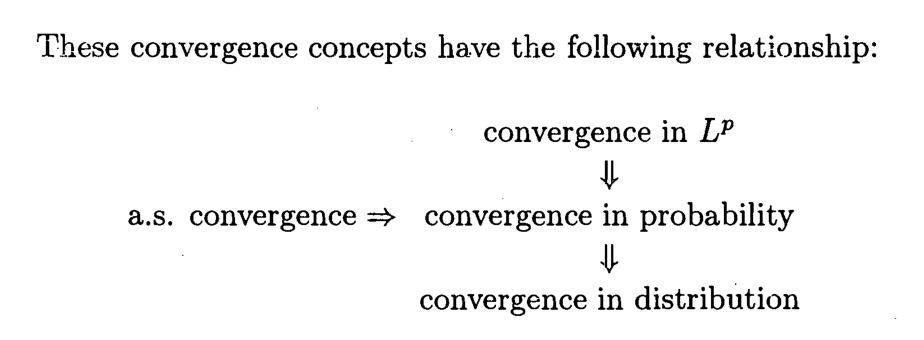
\includegraphics[width=\linewidth]{1}
\label{fig:1}
\end{figure}
\end{frame}

\begin{frame}{随机变量序列依分布收敛}
\begin{equation*}\label{key}
(\Omega,\mathcal{F},P)\xrightarrow{X}(\mathbb{R}^n,\mathcal{B}^n,PX^{-1})
\end{equation*}
随机变量序列依分布收敛的等价定义/条件
\begin{itemize}
\item (重要)分布函数(具体空间的概率测度)弱收敛$ P_nX_n^{-1}\xrightarrow{w}PX^{-1} $

其中,概率测度$ m_n $弱收敛:$ \forall $连续有界$ f $,$ \lim_{n\to\infty}\int_\Omega f\mathrm{d}m_n=\int_\Omega f\mathrm{d}m $

注:分布函数在其他地方常写作$ f_X $或$ \mu_X $,而在本节直接记作$ p $

\item (重要)期望形式:$ \forall $连续有界$ f $,$ \lim_{n\to\infty}\mathbb{E}f(X_n)=\mathbb{E}f(X) $
\item 特征函数$ \varphi(t)=\mathbb{E}(\mathrm{e}^{\mathrm{i}tX}) $点态收敛
\item 随机变量作为对偶空间的元素弱*收敛\footcite{bobrowski_functional_2005}
\end{itemize}
\end{frame}

\begin{frame}{随机过程依分布渐近稳定}
连续情形,由于是渐近稳定性,直接将离散的$ n $换成连续的$ t $即可

由于解有马尔可夫性,分布正好可以由转移概率核表示
\begin{block}{解的马尔可夫性(《SDE》2.8)}
\begin{itemize}
\item 随机微分方程的解是马尔可夫过程(转移概率核$ p(s,x,t,A) $)
\item 若系数满足Lipschitz条件和线性增长条件,则解是强马尔可夫过程(时间可改为停时)
\item 若方程不显含时间$ t $,则解是齐次马尔可夫过程($ p(t,x,A) $)
\end{itemize}
\end{block}

其中由于有Markovian switching,故状态加一个$ i $,于是对任意的$ t,x,i $,分布函数(具体空间的概率测度)的最终形式为$ p(t,(x,i),(\cdot,\cdot)) $
\end{frame}
\begin{frame}{Weak convergence is a metric concept}
书上定义的度量(可能叫Wasserstein度量?)
\begin{gather*}
d_{\mathbb{L}}(p_1,p_2)=\sup_{f\in\mathbb{L}}\Biggl|\sum_{i=1}^{N}\int_{\mathbb{R}^n}f(x,i)p_1(\mathrm{d}x,i)-\sum_{i=1}^{N}\int_{\mathbb{R}^n}f(x,i)p_2(\mathrm{d}x,i)\Biggr|\\
\mathbb{L}=\{f:\mathbb{R}^n\times\mathbb{S}\to\mathbb{R}||f(x,i)-f(y,j)|\le|x-y|+|i-j|,|f(x,i)|\le 1\}
\end{gather*}
之所以是sup而不是inf,是因为本来就是用inf定义的,然后使用对偶原理能转化为sup\footcite{noauthor_wasserstein_2017}

实际上,弱收敛可转化成的度量五花八门,各种讲概率的书(如著名的\footcite{durrett_probability_2019})都会涉及一两个,专著\footcite{rachev_methods_2013}非常全面地研究了各种度量
\end{frame}

\begin{frame}{期望形式}
\begin{align*}
&d_{\mathbb{L}}(p(t,(x,i),(\cdot,\cdot)),p(t,(y,j),(\cdot,\cdot)))\\
={}&\sup_{f\in\mathbb{L}}\Biggl|\sum_{i=1}^{N}\int_{\mathbb{R}^n}f(z,l)p_1(t,(x,i),(\mathrm{d}z,l))-\sum_{i=1}^{N}\int_{\mathbb{R}^n}f(z,l)p_2(t,(y,j),(\mathrm{d}z,l))\Biggr|\\
={}&\sup_{f\in\mathbb{L}}\Biggl|\int_{\mathbb{R}^n\times\mathbb{S}}f(z,l)\mathrm{d}p_1(t,(x,i),(z,l))-\sum_{i=1}^{N}\int_{\mathbb{R}^n}f(z,l)\mathrm{d}p_2(t,(y,j),(z,l))\Biggr|\\
={}&\sup_{f\in\mathbb{L}}\Biggl|\mathbb{E}f(X^{x,i}(t),r(t))-f(X^{y,j}(t),r(t))\Biggr|\\
\end{align*}

\end{frame}

\begin{frame}{概率测度族的“紧性”}
由于定义了度量,此处概率测度处于一个度量空间中,概率测度族$ \{P_t|t\in\Gamma\} $即为其中一个子集,于是可以对其作出拓扑上的要求

\begin{block}{“紧性”}
胎紧(tight):$ \forall\epsilon $,$ \exists $紧集$ K $,$ \forall t\in\Gamma $,$ P_t(K)\ge 1-\epsilon $

相对紧(relatively compact):闭包为紧/对集合中的任意序列,都存在子列收敛于整个空间中某点
\end{block}

Prohorov定理\footcite{karatzas_brownian_1998}:完备可分度量空间(Polish空间)中,胎紧$ \leftrightarrow $相对紧;

可分度量空间中,胎紧$ \rightarrow $相对紧

本节出现的概率测度族胎紧性可由Chebyshev不等式保证,但更一般的情形下需要仔细证明\footcite{du_stability_2014}
\end{frame}

\begin{frame}{本节结构}
\begin{figure}
\centering
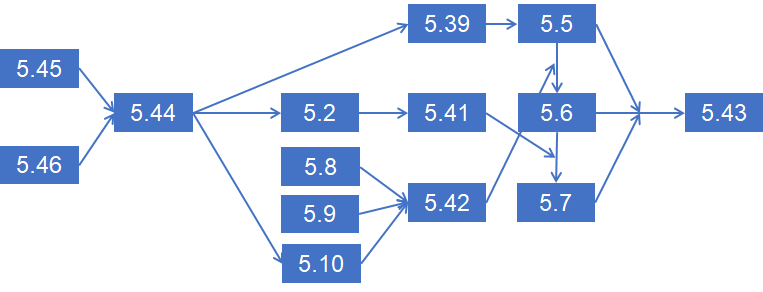
\includegraphics[width=\linewidth]{2}
%\caption{}
\label{fig:2}
\end{figure}

\end{frame}
\end{document}
